\documentclass{article}
\usepackage{mathtools}
\usepackage{amsfonts}
\usepackage{float}


\title{Number of Lobes in Azimuthal Far-field Directivity Pattern of a Uniformly Spaced Delay-and-Sum Beamforming Microphone Array}
\date{12-2016}
\author{Steven Muscari}

\begin{document}
\pagenumbering{arabic}
\numberwithin{equation}{section}
\maketitle

\begin{abstract}
  I investigate the behavior of azimuthal far-field directivity patterns for $N$ mic
  delay-and-sum beamforming microphone arrays with fixed uniform spacing $d$ under
  varying angular frequency $\omega$ and pointing angle $\phi'$. I show that for an
  $N=3$ mic array the number of lobes increases for signals with increasing $\omega$
  and remains the same at fixed $\omega$ for different pointing directions $\phi'$.
\end{abstract}

\section{Introduction}

  While working on the SoundSelect Array System, I picked up most of my
  knowledge of beamforming from McOwan's \emph{Microphone Arrays: A Tutorial} \cite{mccowan}.
  In that time, I observed interesting behavior in what our group referred to as the pick-up
  patterns (see section 2) of our array designs. Further investigation of the behavior was not
  exactly necessary to complete the project. So I set the problem of investigating that behavior aside
  until now, a little over a year past that project's completion. This paper gives a rough explanation of
  my findings so far. I now take the liberty of using the royal we to make reading the maths bearable.

  \begin{figure}[ht]
    \centering
    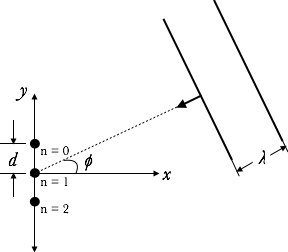
\includegraphics[scale=0.5]{fig1}
    \caption{An $N=3$ mic array along the $y$-axis with incoming wavefronts at and angle $\phi$
             measured from the $x$-axis. The dark circles represent ideal omnidirectional mic elements.
             The dark parallel lines represent incoming wavefronts.}
  \end{figure}

  We begin by deriving the far field directivity for a passive beamforming microphone array
  as shown in figure 1. In the \emph{far field}, we assume all incoming waves are plane waves, perpendicular
  to the $x$-$y$ plane. As such we model our signal $x(t)$, which for the sake of simplicity we consider to be
  a pure sine tone, as a series of wavefronts propagating across the $x$-$y$ plane. We model each
  microphone as an ideal omnidirectional mic element which exactly captures the signal the instant it
  passes over the mic. We arrange $N$ mic elements in a line fixed along the $y$-axis, label them $n = \{0,1,2,\dots,N \}$ as in
  figure 1, and continuosly sum the signal seen be each mic, dividing each signal by $\frac{1}{N}$ to
  keep unity gain, resulting in the output:
  $$ y(t) = \frac{1}{N} \displaystyle\sum_{n=0}^{N-1} x_n (t) $$
  where $x_n (t)$ is the signal seen by mic $n$. Next we consider a single wavefront arriving at some
  variable angle $\phi$.

  Depending on the angle of arrival $\phi$, there will be some delay between the
  arrival of the wavefront at each microphone.
  We see that if the wavefront is traveling perpendicular to
  the $y$-axis from the positive $y$ direction, i.e. $\phi = \frac{\pi}{2}$, the delay for mic $n$ is given
  by $\tau = \frac{nd}{c}$ where $d$ is the mic spacing and $c$ is the speed of sound.
  On the other hand, if the wavefront is parallel to the $y$-axis and arriving from the positive $x$ direction,
  i.e. $\phi = 0$, the wavefront arrives at each mic at the same time, hence the delay for each mic is zero.
  Using these boundary conditions, we can guess that the delay for mic $n$ is given by
  \begin{equation}
    \tau_n = \frac{nd}{c} \sin{\phi}.
  \end{equation}
  By way of a geometric proof, which I won't outline here, one can prove that this indeed gives the delay.

  We now see that $x_n (t) = x(t - \tau_n)$, where $x(t)$ is simply the original signal. Rewriting the output,
  and taking its Fourier transform:
  $$ y(t) = \frac{1}{N} \displaystyle\sum_{n=0}^{N-1} x(t-\tau_n) \xrightarrow{\mathcal{F}} Y(\omega) = \frac{1}{N} \displaystyle\sum_{n=0}^{N-1} X(\omega) e^{i \omega \tau_n} $$
  we arrive at the far field directivity of a passive beamforming mic array:
  \begin{equation}
    D(\omega,\phi) := \frac{1}{N} \displaystyle\sum_{n=0}^{N-1} e^{i \frac{\omega}{c} nd (\sin{\phi})}
  \end{equation}
  Note that this is simply the system response of the array to a signal $X(\omega)$.

  In order to turn this system into an \emph{active} beamforming array, i.e. an array with a \emph{virtual}
  pointing direction $\phi'$, we simply augment the passive system response with a factor
  $$ D_n (\omega, \phi') = e^{-{i \frac{\omega}{c} nd (\sin{\phi'})}}. $$
  This effectively tricks the mic array into thinking it has been rotated by some angle $\phi'$ in the $x$-$y$ plane,
  even though it's still fixed along the $y$-axis. The new far field directivity is given by
  \begin{equation}
    D(\omega,\phi,\phi') = \frac{1}{N} \displaystyle\sum_{n=0}^{N-1} e^{i \frac{\omega}{c} nd (\sin{\phi} - \sin{\phi'})}.
  \end{equation}
  And the new output is $$Y(\omega, \phi, \phi') = X(\omega) D(\omega,\phi,\phi').$$
  We choose to have the negative sign in the exponential in $D_n (\omega,\phi)$ so that when
  $\phi = \phi'$, $Y(\omega, \phi, \phi') = X(\omega)$, i.e. when the array is virtually pointed towards the direction of arrival of the incoming signal,
  the output is the original signal.

\section{Exploring the Far-field Directivity Pattern}

One can plot the magnitude gain of the directivity of a beamforming mic array in polar coordinates to get a sense
of how the array picks up sound from different angles. Hence we colloquially refer to these plots as \emph{pick-up
patterns}, although they are formally known as directivity patterns. Figure 2
shows some sample pick-up patterns of a beamforming array in the plane. These plots are in decibels
where the maximum possible gain is unity. We call the local maxima in these plots \emph{lobes}. (We should add that, because
our design was to be wall mounted, we most often ignored the half of the plane where $x<0$, i.e. we assumed the wall on which
the system was mounted neither reflected nor transmitted sound.)

\begin{figure}[ht]
  \centering
  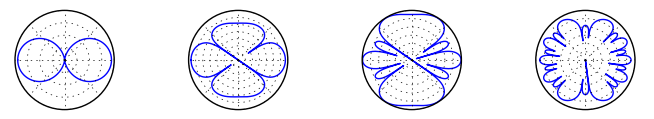
\includegraphics[scale=0.5]{omegas}
  \caption{The polar directivity pattern for an $N = 3$ passive mic array at
           increasing signal frequency $\omega$ from left to right.}
\end{figure}


Notice that as the frequency increases, the number of lobes in the pick-up pattern also increases.
This is a not-so-surprising result of spatial aliasing. The mic spacing $d$ is held constant,
so we expect that for signal above a certain frequency $\omega$ (or below a certain wavelength $\lambda$)
our mic array undersamples the signal. It can be shown that this wavelength $\lambda^{*} = 2d$ \cite{mccowan}. This
gives the critical frequency $\omega^{*} = \frac{\pi c}{d}$ above which sound can alias into our signal from a
direction other than the pointing direction $\phi'$.
\begin{figure}[ht]
  \centering
  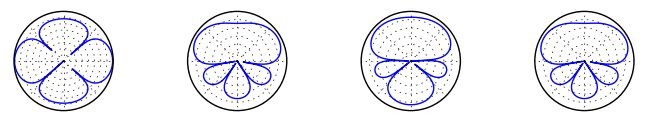
\includegraphics[scale=0.5]{omega_money_4_lobes}
  \caption{The polar directivity pattern for an $N = 3$ passive mic array at
           the center frequency $\omega^{*} = \frac{\pi c}{d}$. The point angle $\phi'$
           increases from $0$ to $\frac{5\pi}{6}$ from left to right. Notice that
           there are 4 lobes in each pattern.}
\end{figure}

Figure 3 shows pick-up patterns for signal fixed at $\omega^{*}$ for varying pointing angles $\phi'$.
\emph{The interesting observation referred to in the introduction is
that the number of lobes remains unchanged for different} $\phi'$. See figure 4 for more examples of this.
In the next section we investigate why this is for the case where $N=3$.
\begin{figure}[H]
  \centering
  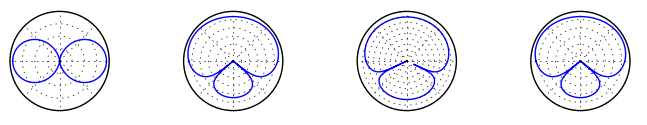
\includegraphics[scale=0.5]{omega1_2_lobes}
  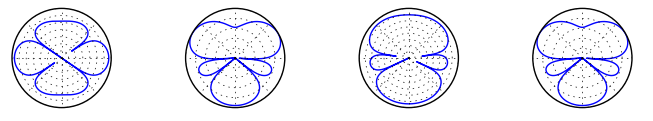
\includegraphics[scale=0.5]{omega2_6_lobes}
  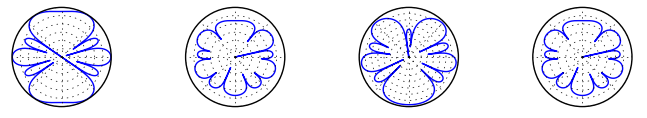
\includegraphics[scale=0.5]{omega3_10_lobes}
  \caption{The polar directivity pattern for an $N = 3$ passive mic array at
           increasing signal frequency $\omega$ from top to bottom and increasing
           pointing angle from left to right. Notice that the number of lobes does not
           change at fixed frequecy does not change. Each pattern has two lobes in row 1,
           6 lobes in row 2, and 10 lobes in row 3.}
\end{figure}

\section{The $\omega$ and $\phi'$ Dependence of Directivity in a $N=3$ Mic Array}
We first investigate the $\omega$ dependence of equation 1.3. Expanding the sum with $N=3$, differentiating with
respect to $\omega$, setting the result equal to zero, and rearranging some factors we obtain
\begin{equation}
  \frac{N}{\alpha} \frac{\partial}{\partial \omega} D(\omega, \phi, \phi') = 1 + 2e^{i\omega \frac{d}{c} \alpha} = 0,
\end{equation}
where $\alpha := \sin{\phi}-\sin{\phi'}$. Using Euler's Formula we find the solutions of equation 3.1 satisfy
$$ \cos\Big( \frac{\omega d \alpha}{c} \Big) = - \frac{1}{2} $$ or, substituting back $\sin{\phi}-\sin{\phi'}$ for $\alpha$ and
solving for $\phi$, we find the equation
\begin{equation}
  \phi_m = \arcsin \Big[ \frac{c}{\omega d} \frac{2}{3} (3m \pm 1) \pi + \sin{\phi'} \Big],\ m \in \mathbb{Z},
\end{equation}
which has an integer number of solutions $M$.

\section{Conclusion}
Exlporing the values of $D(\omega,\phi,\phi')$ around $\phi_m$, we find that the $M$ valid solutions for $\phi_m$ give the location of
the local minima of $D(\omega,\phi,\phi')$ on the interval $\phi \in [-\pi/2,\pi/2]$ where we use symmetry along the $y$-axis to complete
the directivity pattern. This allows us to write an expression for the number of lobes at fixed frequency $\omega$,
\begin{equation}
  N_{\text{lobes}} = 2(M-1).
\end{equation}
Further inspection of equation 3.2 reveals that as the signal frequency $\omega$ increases, the
number of possible $\phi_m$, $M$, also increases in agreement with the findings of section 2. One can also glean from equation
3.2 that there exists a frequency $\omega$ below which there will be no local minima, which also must be true since for
signals with sufficiently large wavelength $\lambda \gg d$ our mic array behaves as a single mic element.

Finally, we also see from equation 3.2 that varying $\phi'$ alters the position of the various $\phi_m$ but it does nothing
to change the total number of minima $M$ for fixed frequency $\omega$.

This, of course, only covers the $N=3$ case. For $N>3$ we could follow a similar approach to that of section 3. But it
would be nice to find a more general method to explore this behavior for all $N$.


\bibliography{lobesbib}
\bibliographystyle{ieeetr}

\end{document}
